\documentclass{wseminar}
\title{Wandel des Energieverbrauchs im digitalen Alltag}
\author{Paul Deininger}
\date{ 07.11.2023 }

\makeglossaries

\loadglsentries{abkuerzungen}

\begin{document}
\begin{sloppypar}
    \maketitle
    \thispagestyle{empty}   % no page number
    \pagebreak
    %\setcounter{page}{1}    % Falls Deckblatt nicht Seite 1 sein soll: am Anfang der Zeile '%' entfernen
    \tableofcontents        % Inhaltsverzeichnis
    \thispagestyle{empty}   % no page number
    \pagebreak

    % Hier beginnen zu bearbeiten


    \section{Digitalisierung der Welt}	
    
	\pagebreak
	
	
	
	\section{Energieeffizienz im Remoteoffice}	
	Das Remoteoffice oder Homeoffice lässt sich auf viele verschiedene Weisen gestalten.
Der Mitarbeiter kann an einem eigenen Laptop arbeiten und dabei offline sein, oder er benötigt zur Arbeit dauerhaft eine Internetverbindung, da sein Laptop lediglich als Peripheriegerät dient.
Bei letzterem Fall kann der Energieverbrauch des Laptops erheblich gesenkt werden, die damit verbundenen Vorteile werden im Folgenden erläutert.
Davor sollen jedoch drei extrem Fälle visualisiert werden:
\begin{figure}[!htb]
    \captionsetup{width=.8\linewidth}
    \includegraphics[height=.3\linewidth]{images/virtualization/no}
    \centering
    \caption{Desktop-PC: Ein unabhängiger Computer, welcher von dem Endnutzer alleine genutzt wird.}
    \label{fig:virt-no}
\end{figure}\\
\begin{figure}[!htb]
    \captionsetup{width=.8\linewidth}
    \includegraphics[width=.8\linewidth]{images/virtualization/thin}
    \centering
    \caption{Thin Client: Ein Laptop oder Mini-PC der mit einem Terminal-Server verbunden ist.}
    \label{fig:virt-thin}
\end{figure}\\
% TODO: Übergang
Der Terminal-Server übernimmt dabei die Rechenarbeit der Anwendungen des Thin Clients.
Manchmal wird auch das komplette Betriebssystem des Thin Client auf dem Server ausgeführt.
Der genaue Aufbau soll hier nicht diskutiert werden, aber der energetische Aspekt, welcher je nach Aufbau unterschiedlich ist.\
Bei dem extrem Fall, bei welchem der Thin Client wirklich nur als Peripheriegerät dient, wird trotzt alle dem ein minimales Betriebssystem für die Internetverbindung ausgeführt.
Dieses kann dadurch deutlich weniger Ressourcen benötigen und selbst eine Größe unter 100 MB\citeurl{tiny-core} haben, im Gegensatz zu Windows 10(c), welches eine Festplatte mit über 20 GB\footnote{Dies habe ich selber durch ausprobieren mit einer Virtuellen Maschine festgestellt} Speicherplatz verlangt.   % kein guter Beleg, da innerhalb des Installers /    % Github letzte Änderung vor wenigen Minuten => aktive Entwicklung und builds von diesem Jahr
Da das eigentliche Betriebssystem von mehreren dann auf ein und demselben Server gespeichert sind können hier verschiedene Optimierungen, wie \gls{copy-on-write} oder \gls{disp-vm} verwendet werden.
Diese sparen Speicherplatz und damit Energie, aber die meiste Energie wird gespart durch eine nun mögliche nahezu vollständige Auslastung des Servers im Gegensatz zu vielen nicht annähernd vollständig ausgelasteten Laptops.
Hierbei kann Load Balancing eingesetzt werden, wenn auf dem Terminalserver die weiter unten beschriebene Vollständige Virtualisierung und oder Betriebssystem-Virtualisierung eingesetzt wird.
[...]
Es wird davon ausgegangen, dass schätzungsweise 30\% der Büro-PCs in Großbritannien nicht abgeschaltet werden\citebook[130]{green-it} und nur sechs bis 25\% der Büro-Computer mit einem Powermanagement betrieben werden (GreenIT S.129).
Allein dies zeigt, dass hier eine Zentralisierung von Vorteil ist, diese sorgt für eine CO2einsparung von durchschnittlich 44\% bei Verwendung von Thin Clients. Diese Einsparung lässt sich direkt auf den Energieverbrauch übertragen, da zur Ermittlung der CO2Emissionen während dem Betrieb ausschließlich der Stromverbrauch berücksichtigt wurde. (Green IT S.132)
Insgesamt kann über den gesamten Lebenszyklus so 56\% CO2 gespart werden \autoref{table:cont}, die gesparte Energie wird geringfügig abweichen, aufgrund der nicht ausschließlich auf Energie beruhenden Zahlen.
\begin{table}
    \centering
\csvreader[
  separator=semicolon,
  % l = column: left-aligned c -> centered r -> rihgt
  tabular=|l|c|c|c|r|,
  % header names (first row of csv is skipped) header name in {} and between two of them '&'
  % for bold header names add '\bfseries' before
  table head=\hline \bfseries{} & \bfseries{Desktop-PC} & \bfseries{Thin Client} & \bfseries{T. C. + Serveranteil} & \bfseries{Differenz} \\\hline,
  late after last line=\\\hline % horizontal line at the end of the table
  % dateipfad
]{tables/co2-virtualisation.csv}{}{\csvlinetotablerow}
\caption{Tabelle mit Daten aus: \citebookinline[131]{green-it}}
\label{table:cont}
\end{table}\\
	\pagebreak
	
	
	
	\section{Neuronale Netze}	
	
	\pagebreak
	
	
	
	\section{Entertainment}	
	
	\pagebreak
	
	
	
	\section{Rficient(c)}	
	
	\pagebreak
	
	
	
	\section{Geld / Gruen}	

	\pagebreak
	
	
	
	\section{Intelligente Systeme}	
	
	\pagebreak
	
	
	
	\section{Einigungsalgorithmen}	
	
	\pagebreak
	
	
	
	\section{Schluss}
	
	\pagebreak
	
	
	
	\section{Anhang}

	\pagebreak
	
	
	
	\section{Abkuerzungsverzeichnis}
        \printunsrtglossaries % list all entries    % Zur Beschleunigung Auskommentieren
        % erst am Ende das '%' entfernen, um Vorschau schneller zu generieren
	\pagebreak
	
	
	
	\section{Literaturverzeichnis}
        \printbibliography  % Zur Beschleunigung Auskommentieren
        % erst am Ende das '%' entfernen, um Vorschau schneller zu generieren
	\pagebreak
	
	
	
	\section{Eidesstattliche Erklaerung}	
	
	\pagebreak
\end{sloppypar}
\end{document}